\section{Blockchain Ethereum et smart contracts}
\framewithtitle{Blockchain Ethereum et smart contracts}

\begin{frame}{Sommaire}
  \setcounter{tocdepth}{2}
  \tableofcontents[currentsection, hideothersubsections]
\end{frame}

\begin{frame}{Objectifs de ce module}
  Comprendre les opérations de base de la cryptographie
  \begin{enumerate}
    \item Interagir avec une blockchain de test (Ethereum Sepolia)
    \item Interagir avec une blockchain de production (Polygon)
  \end{enumerate}
\end{frame}

\begin{frame}{Créer un wallet avec MetaMask}
  \begin{columns}
    \begin{column}{0.7\textwidth}
      \begin{itemize}
        \item Ceux qui on déjà un wallet : bonne sieste
        \item Les autres, installez l'extension MetaMask sur votre navigateur (Chrome / Firefox)
        \item Effectuez l'onboarding et notez bien la phrase de récupération
      \end{itemize}
    \end{column}
    \begin{column}{0.25\textwidth}
      \begin{figure}
        \resizebox{\textwidth}{!}{
          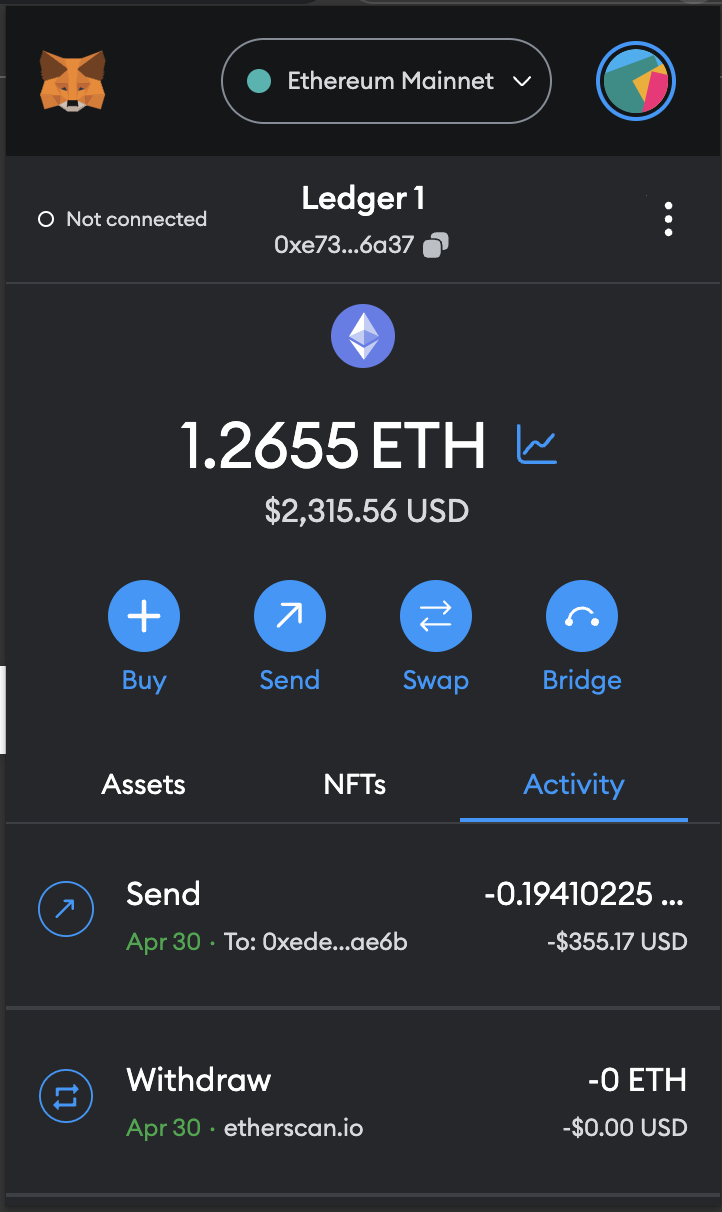
\includegraphics{img/metamask.png}
        }
      \end{figure}
    \end{column}
    \begin{column}{0.05\textwidth}\end{column}
  \end{columns}
\end{frame}

\begin{frame}{Seed phrase}
  Lors de la création d'un wallet avec MetaMask, une phrase de douze mots est générée.

  \begin{center}
    \begin{tcolorbox}[arc=1ex, colback=myuniversity, colframe=myuniversity, left=3pt, right=3pt, top=3pt, bottom=2pt]
      \vspace*{1cm}
      \begin{center}
        \begin{huge}
          \textcolor{white}{
            Il faut absolument la sauvegarder en lieu sûr.\\
            Quiconque l'obtient peut accéder à tout votre wallet, vos cryptos et vos NFTs !
          }
        \end{huge}
      \end{center}
      \vspace*{1cm}
    \end{tcolorbox}
  \end{center}
\end{frame}

\begin{frame}{Notion de gas}
  \begin{itemize}
    \item Contrairement à la blockchain Bitcoin, les frais Ethereum ne paie pas à la transaction mais à la complexité du calcul
    \item Transférer de l'Ether entre deux comptes est beaucoup moins coûteux que faire participer à une enchère de NFTs
    \item La complexité des transactions en Ethereum se mesure en \textquote{gas}
    \item L'utilisateur peut choisir le prix du gas affecté à sa transaction.
    \item Le gas se mesure en Gwei avec 1 ETH = 1000000000 Gwei
  \end{itemize}
\end{frame}
\subsection{Développer des contrats avec Foundry}
\framewithtitle{Foundry}

\begin{frame}{Foundry}
  Dans ce cours, nous allons utiliser Foundry, un utilitaire permettant de développer des smart-contracts simplement.
\end{frame}

\begin{frame}[fragile]{Installation de Foundry : Windows}
  Il faut d'abord installer Windows Subsystem Linux avec :
  \begin{minted}{bash}
    $ wsl --install
  \end{minted}

  WSL demandera de redémarrer, puis au redémarrage de choisir un nom d'utilisateur et un mot de passe.
  Pour confirmer la bonne installation de WSL, exécuter :

  \begin{minted}{bash}
    $ wsl --list
  \end{minted}
\end{frame}

\begin{frame}[fragile]{Installation de Foundry}
  Configurer git avec votre nom / email :

  \begin{minted}{bash}
    $ git config --global user.email "you@example.com"
    $ git config --global user.name "Prénom Nom"
  \end{minted}

  Installer Foundryup (installateur de Foundry)
  \begin{minted}{bash}
    $ curl -L https://foundry.paradigm.xyz | bash
  \end{minted}

  Redémarrer le terminal, lancer Foundryup
  \begin{minted}{text}
    $ foundryup
  \end{minted}

  Redémarrer le terminal, lancer Forge
  \begin{minted}{text}
    $ forge
    forge 0.2.0 (31fcf5a 2023-05-19T00:10:33.861185000Z)
  \end{minted}
\end{frame}

\begin{frame}{Architecture d'un projet Foundry}
  \dirtree{%
    .1 /.
    .2 out\DTcomment{Fichiers compilés}.
    .2 lib\DTcomment{Libraries installées}.
    .2 src\DTcomment{Code source des contrats}.
    .2 test\DTcomment{Test des contrats}.
    .2 .gitmodules.
    .2 foundry.toml\DTcomment{Configuration de Foundry}.
  }
\end{frame}
\framewithtitle{Solidity}

\begin{frame}{Qu'est-ce qu'un smart contract}
  \begin{block}{Définition : smart contract}
    Sur la blockchain Ethereum, un smart contract est un bytecode (=code hexadécimal) associé à une adresse.

    $\Rightarrow$ Les adresses des smart contracts sont indiscernables des adresses des comptes utilisateurs.
  \end{block}

  \begin{block}{Définition : Externally Owned Account}
    Les adresses contrôlés par des utilisateurs sont appelées \enquote{Externally Owned Account} (EOA).
  \end{block}

  Voir le glossaire d'Ethereum: \url{https://ethereum.org/en/glossary}
\end{frame}

\begin{frame}{Solidity ?}
  \begin{block}{Définition : Solidity}
    Solidity est un \textbf{langage de programmation} utilisé pour écrire des smart contracts sur la plateforme Ethereum.

    Solidity permet aux développeurs de définir des règles et des logiques spécifiques à un smart contract.
    Il permet d'écrire des lignes de code qui définissent comment un smart contract doit fonctionner, quelles actions il doit effectuer et comment il doit réagir dans différentes situations.

    En utilisant Solidity, les développeurs peuvent créer des smart contracts pour diverses applications décentralisées (dApps)
  \end{block}
\end{frame}

\begin{frame}[fragile]{Solidity : syntaxe en POO}
  \begin{minted}{solidity}
    // SPDX-License-Identifier: UNLICENSED
    pragma solidity ^0.8.13;
    
    contract Counter {
        uint256 public number;
    
        function setNumber(uint256 newNumber) public {
            number = newNumber;
        }
    }
  \end{minted}
\end{frame}

\begin{frame}[fragile]{Solidity : header}
  Le header d'un smart contract s'écrit en deux lignes :

  \begin{minted}{solidity}
    // SPDX-License-Identifier: UNLICENSED
    pragma solidity ^0.8.13;
  \end{minted}

  La ligne 1 défini la licence du fichier :

  \begin{itemize}
    \item \solidity{UNLICENSED} signifie que le code est complètement privé
    \item \solidity{pragma solidity ^0.8.13;} version de Solidity compatible avec le fichier
  \end{itemize}
\end{frame}

\begin{frame}{Semantic versionning}
  \begin{block}{Semantic versionning \enquote{SemVer}}
    Le versionnage sémantique  est une méthode de numérotation des versions logicielles basée sur des règles spécifiques.
    Elle se compose de trois nombres séparés par des points : MAJEUR.MINEUR.PATCH.
    Le numéro MAJEUR est augmenté lorsque des changements incompatibles sont apportés, le numéro MINEUR est augmenté lorsque des fonctionnalités sont ajoutées de manière rétrocompatible, et le numéro PATCH est augmenté pour les corrections de bugs rétrocompatibles.
  \end{block}

  \begin{columns}
    \begin{column}{0.48\textwidth}
      \begin{block}{Opérateurs}
        \begin{itemize}
          \item \texttt{=1.2.3} strictement égal à 1.2.3
          \item \texttt{\^{}1.2.3} $\Rightarrow$ \texttt{1.2.3 < v < 2.0.0}
          \item \texttt{\~{}1.2.3} $\Rightarrow$ \texttt{1.2.3 < v < 1.3.0}
        \end{itemize}
      \end{block}
    \end{column}
    \hspace{0.01\textwidth}
    \begin{column}{0.48\textwidth}
      \begin{block}{Opérateurs (MAJEUR=0)}
        \begin{itemize}
          \item \texttt{=0.1.2} strictement égal à 0.1.2
          \item \texttt{\^{}0.1.2} $\Rightarrow$ \texttt{0.1.2 < v < 0.2.0}
        \end{itemize}

        \vspace{1em}
        \vspace{\smallskipamount}
      \end{block}
    \end{column}
  \end{columns}
\end{frame}

\begin{frame}{Solidity : types primitifs}
  \begin{itemize}
    \item \solidity{uint} un entier non signé sur 256 bits
    \item \solidity{uint8} un entier non signé sur 8 bits
    \item \solidity{uint32} un entier non signé sur 32 bits
    \item \solidity{uint256} un entier non signé sur 256 bits
    \item \solidity{int} un entier signé sur 256 bits
    \item \solidity{int32} un entier signé sur 32 bits
    \item \solidity{address} une adresse Ethereum
    \item \solidity{string} une chaîne de caractères
    \item \solidity{struct} structure, au sens langage C du terme
    \item \solidity{mapping} une association clé-valeur
  \end{itemize}
\end{frame}

\begin{frame}[fragile]{Solidity : le type \texttt{address}}
  Le type \solidity{address} est spécial et possède des propriétés :

  \begin{itemize}
    \item \solidity{<address>.balance} le montant d'ether détenu par l'adresse
    \item \solidity{<address>.code} le code à l'adresse (vide pour les EOA)
    \item Dans un contrat, \solidity{address(this).balance} donne la balance du contrat
  \end{itemize}
\end{frame}

\begin{frame}{Solidity : variables spéciales}
  \begin{block}{\texttt{msg} (= message)}
    Un message représente un appel d'une fonction d'un smart contract.

    \begin{itemize}
      \item \solidity{msg.sender} expéditeur du message
      \item \solidity{msg.value} nombre d'Ether envoyés avec le message
    \end{itemize}
  \end{block}


  \begin{block}{\texttt{block}}
    Metadata du bloc actuel.

    \begin{itemize}
      \item \solidity{block.number} numéro du bloc actuel
      \item \solidity{block.timestamp} tinmestamp UNIX en secondes
    \end{itemize}
  \end{block}
\end{frame}

\begin{frame}[fragile]{Solidity : contrôle de flow}
  \begin{columns}
    \begin{column}{0.47\textwidth}
      \solidity{if} / \solidity{else} / \solidity{else if}

      \begin{minted}{solidity}
        if (cond) {
          // if path
        } else if (cond2) {
          // else if path
        } else {
          // else path
        }
      \end{minted}

      Note : pas de \solidity{switch / case} en Solidity.
    \end{column}
    \vspace{0.03\textwidth}
    \begin{column}{0.47\textwidth}
      \solidity{for} / \solidity{while}

      \begin{minted}{solidity}
        for (uint256 i = 0; i < n; i++) {
          // do stuff
        }

        while(cond) {
          // do other stuff
        }
      \end{minted}

      Note : pas de \solidity{do while} en Solidity.
    \end{column}
  \end{columns}
\end{frame}

\begin{frame}[fragile]{Solidity : visibilité}
  \begin{columns}
    \begin{column}{0.47\textwidth}
      \begin{block}{Public}
        \begin{minted}{solidity}
          uint public myVariable;
          function myFunction() public {
            // Function logic
          }
        \end{minted}
      \end{block}
    \end{column}
    \vspace{0.03\textwidth}
    \begin{column}{0.47\textwidth}
      \begin{block}{Private}
        \begin{minted}{solidity}
          uint internal myVariable;
          function myFunction() internal {
            // Function logic
          }
        \end{minted}
      \end{block}
    \end{column}
  \end{columns}

  \begin{columns}
    \begin{column}{0.47\textwidth}
      \begin{block}{Internal}
        \begin{minted}{solidity}
          uint internal myVariable;
          function myFunction() internal {
            // Function logic
          }
        \end{minted}
      \end{block}
    \end{column}
    \vspace{0.03\textwidth}
    \begin{column}{0.47\textwidth}
      \begin{block}{External}
        \begin{minted}{solidity}
          // external variables not possible 
          function myFunction() external {
            // Function logic
          }
        \end{minted}
      \end{block}
    \end{column}
  \end{columns}
\end{frame}

\begin{frame}[fragile]{Solidity : \texttt{modifier}}
  \begin{block}{Définition : \texttt{modifier}}
    En Solidity, un \enquote{modifier} est une fonction spéciale qui permet de modifier le comportement d'autres fonctions dans un contrat intelligent.
    Les modifiers fournissent un moyen pratique de réutiliser du code et d'ajouter des conditions supplémentaires ou des vérifications avant l'exécution d'une fonction.
  \end{block}


  \begin{block}{Syntaxe : \texttt{modifier}}
    \begin{minted}{solidity}
    modifier exampleModifier() {
      _; // Continue function execution
    }

    function foobar() public exampleModifier {}
  \end{minted}
  \end{block}
\end{frame}

\begin{frame}[fragile]{Solidity : interfaces}
  Comme beaucoup d'autres langages, Solidity dispose d'interfaces\footnote{Voir la \href{https://docs.soliditylang.org/fr/stable/contracts.html\#interfaces}{documentation Solidity des interfaces}} qui servent à intégrer des notions de polymorphisme.

  \begin{itemize}
    \item Elles ne peuvent pas hériter d'autres contrats, mais elles peuvent hériter d'autres interfaces.
    \item Toutes les fonctions déclarées doivent être externes.
    \item Elles ne peuvent pas déclarer de \texttt{constructor}, de variables d'état ou de \texttt{modifier}.
  \end{itemize}

  \begin{block}{Syntaxe : interface}
    \begin{minted}{solidity}
      interface IIoken {
        function transfer(address recipient, uint amount) external;
      }
    \end{minted}
  \end{block}
\end{frame}

\begin{frame}[fragile]{Solidity : events}
  \begin{itemize}
    \item La blockchain est \enquote{isolée} du monde extérieur : impossible de contacter le monde extérieur (pas de requête HTTP, notifications, etc.).
    \item Solidity permet de définir des events qui peuvent être écoutés à l'extérieur de la blockchain.
  \end{itemize}

  \begin{minted}{solidity}
    // Event declaration
    event Minted(address indexed to, uint256 amount);

    function transfer(address to, uint256 amount) {
      balanceOf[to] += amount;
      emit Minted(to, value); // Event emission
    }
  \end{minted}

  \begin{minted}{typescript}
    client.watchEvent({
      address: '0xa0b86991c6218b36c1d19d4a2e9eb0ce3606eb48',
      event: parseAbiItem('event Minted(address indexed to, uint256 amount)'), 
      onLogs: logs => console.log(logs)
    })
  \end{minted}
\end{frame}

\begin{frame}[fragile]{Solidity : events indexed}
  Les events peuvent avoir certains de leurs arguments marqués comme \solidity{indexed}.
  Cela permet de filtrer sur les valeurs ces arguments.

  Exemple : \solidity{event Transfer(address indexed from, address indexed to, uint256 value)}.

  \begin{itemize}
    \item Si on considère deux addresses \texttt{x} et \texttt{y}:
    \item Il est possible d'écouter les transactions émises par \texttt{x}
    \item Il est possible d'écouter les transactions reçues par \texttt{x}
    \item Il est possible d'écouter les transactions émises par \texttt{x} vers \texttt{y}
    \item Il n'est pas possible d'écouter les transactions de 1 ETH ou moins car \solidity{uint256 value} n'est pas \solidity{indexed}.

  \end{itemize}
\end{frame}

\begin{frame}[fragile]{Solidity : erreurs}
  Souvent, il faut arrêter l'exécition d'un smart contract et renvoyer une erreur (exécution non autorisée, opération impossible, etc.).

  \begin{columns}
    \begin{column}{0.47\textwidth}
      Fonction \solidity{revert(bool assertion, string message)}

      Revert si \solidity{assertion} est évalué à false.
    \end{column}
    \vspace{0.01\textwidth}
    \begin{column}{0.47\textwidth}
      Custom errors: permet de déclarer des erreurs avec des paramètres.

      \begin{minted}{solidity}
        contract Foo {
          error Custom(uint256 arg1);

          function willRevert() public {
            revert Custom(1);
          }
        }
      \end{minted}
    \end{column}
  \end{columns}
\end{frame}

\begin{frame}[fragile]{Exemple : cryptomonnaie avec mint initial}
  \begin{minted}{solidity}
    contract Mewo {
      uint256 constant MAX_SUPPLY = 1000000000; // 1 billion
      mapping(address => uint256) public balances;

      contructor() {
        balances[msg.sender] += MAX_SUPPLY; // Initial mint
      }

      function transfer(address to, uint256 amount) public {
        require(balances[msg.sender] >= amount, "Insufficient balance");
        balances[msg.sender] -= amount;
        balances[to] += amount;
      }
    }
  \end{minted}
\end{frame}

\begin{frame}[fragile]{Exemple : cryptomonnaie}
  \begin{minted}{solidity}
    contract Mewo {
      mapping(address => uint256) public balances;

      function transfer(address to, uint256 amount) public {
        require(balances[msg.sender] >= amount, "Insufficient balance");
        balances[msg.sender] -= amount;
        balances[to] += amount;
      }
    }
  \end{minted}
\end{frame}

\begin{frame}[fragile]{Exemple : cryptomonnaie avec mint}
  \begin{minted}{solidity}
    contract Mewo {
      mapping(address => uint256) public balances;

      function mint(uint256 amount) public {
        balances[msg.sender] += amount
      }

      function transfer(address to, uint256 amount) public {
        require(balances[msg.sender] >= amount, "Insufficient balance");
        balances[msg.sender] -= amount;
        balances[to] += amount;
      }
    }
  \end{minted}
\end{frame}

\begin{frame}[fragile]{Exemple : cryptomonnaie avec mint protégé}
  \begin{minted}{solidity}
    contract Mewo {
      address owner;
      mapping(address => uint256) public balances;

      constructor() {
          owner = msg.sender;
      }
    
      modifier onlyOwner() {
          require(msg.sender == owner, "Only owner");
          _;
      }
    
      function mint(uint256 amount) public onlyOwner {
          balances[msg.sender] += amount;
      }
    }
  \end{minted}
\end{frame}

\begin{frame}{Notion de gas}
  \begin{itemize}
    \item Les frais Ethereum ne paie pas à la transaction mais à la \textbf{complexité du calcul}
    \item Transférer de l'Ether entre deux comptes est beaucoup moins coûteux que faire participer à une enchère de NFTs
    \item La complexité des transactions en Ethereum se mesure en \enquote{gas}
    \item Le prix d'un \enquote{gas} se mesure en Gwei avec 1 ETH = 1000000000 Gwei.
    \item L'utilisateur peut choisir le prix du \enquote{gas} affecté à sa transaction.
  \end{itemize}

  \begin{block}{Exemple : \texttt{Mewo.mint}}
    \begin{itemize}
      \item Gas utilisé pour la fonction mint : $24634$
      \item Prix du gas : $37$ gwei/gas
      \item Prix d'un ETH = \$1,817.85
      \item Total = $24634\times37=911458$ gwei $= 0.000911458$ ETH $ = \$1.657$
    \end{itemize}
  \end{block}
\end{frame}
